\documentclass[12pt,a4paper]{article}
\usepackage{fontspec}
\IfFontExistsTF{Times New Roman}{\setmainfont{Times New Roman}}{\setmainfont{CMU Serif}}
\usepackage[russian]{babel}
\usepackage[margin=18mm]{geometry}
\usepackage{amsmath,amssymb,graphicx,booktabs,tabularx,caption,titlesec}
\usepackage[unicode,hidelinks]{hyperref}
\titlespacing*{\section}{0pt}{9pt}{4pt}
\titlespacing*{\subsection}{0pt}{6pt}{3pt}
\setlength{\parindent}{1cm}
\setlength{\emergencystretch}{2em}
\setlength{\abovedisplayskip}{5pt}
\setlength{\belowdisplayskip}{5pt}
\captionsetup{font=small,skip=4pt}
\newcommand{\resultstrip}[2]{\begin{center}\begin{minipage}{\linewidth}\centering\includegraphics[width=\linewidth]{results/#1-comparison.png}\captionof{figure}{#2}\end{minipage}\end{center}}
\makeatletter\setlength{\@fptop}{0pt}\makeatother
\begin{document}
\begin{center}
{\large\bfseries Лабораторная работа №2}\\
Основы обработки цифровых изображений\\
Ходько Мария Дмитриевна, группа 3, вариант 12
\end{center}

\section{Цель и задание}
Изучить и реализовать методы обработки изображений, сравнить их на подходящих примерах и разработать приложение с графическим интерфейсом.

Порядковому номеру 12 соответствует третья строка и второй столбец таблицы вариантов: локальная пороговая обработка (два метода с их сравнением) и низкочастотные сглаживающие фильтры. Реализованы локальное среднее с вычитанием константы, метод Сауволы, усредняющий и гауссов фильтры. Сжатие в выбранный вариант не входит.

\section{Алгоритмы}
\subsection{Подготовка изображения}
Цветное изображение переводится в яркость:
\[I(x,y)=0.299R(x,y)+0.587G(x,y)+0.114B(x,y).\]
Прозрачность предварительно накладывается на белый фон. Яркость хранится в диапазоне 0--255. Изображения с максимальной стороной более 1280 пикселей пропорционально уменьшаются; пользователь видит сообщение и фактические размеры.

\subsection{Локальная пороговая обработка}
Для каждого пикселя вычисляется порог по квадратному окну $\Omega$ нечётного размера $N\times N$. Если $n$ --- фактическое число пикселей окна, то
\[m=\frac1n\sum_{(i,j)\in\Omega} I(i,j),\qquad s=\sqrt{\max\left(0,\frac1n\sum_{(i,j)\in\Omega}I(i,j)^2-m^2\right)}.\]
На границах окно обрезается до доступной части изображения, а нормировка выполняется по фактическому числу пикселей.

\textbf{Локальное среднее:} $T_{\mathrm{mean}}(x,y)=m(x,y)-C$. Константа $C$ задаёт отступ от средней яркости. Увеличение $C$ уменьшает число чёрных пикселей: фон очищается, но слабые штрихи могут исчезать. Формула соответствует подходу adaptive mean, описанному в документации OpenCV; побитовая совместимость с OpenCV не заявляется, поскольку обработка границ и округление могут различаться.

\textbf{Метод Сауволы:}
\[T_{\mathrm{Sauvola}}(x,y)=m(x,y)\left[1+k\left(\frac{s(x,y)}{R}-1\right)\right],\qquad R=128.\]
Коэффициент $k$ регулирует влияние локального разброса яркости. При $s<R$ увеличение $k$ понижает порог и уменьшает число чёрных пикселей. Это помогает подавить фактуру светлого фона, но может удалить бледный текст.

Для обоих методов используется одно правило бинаризации:
\[B(x,y)=\begin{cases}255,&I(x,y)>T(x,y),\\0,&I(x,y)\le T(x,y).\end{cases}\]
Тёмный текст считается объектом, белый цвет --- фоном. Одного глобального порога нет: порог меняется для каждого пикселя.

Среднее и дисперсия рассчитываются через интегральные изображения суммы и суммы квадратов. Сумма любого прямоугольного окна получается четырьмя обращениями к таблице. Подготовка и обработка изображения имеют сложность $O(WH)$; размер окна не увеличивает число операций на пиксель. Промежуточные суммы хранятся в Float64.

\subsection{Низкочастотные фильтры}
\textbf{Усредняющий фильтр} заменяет пиксель средним значением яркости в окне:
\[J_{\mathrm{box}}(x,y)=\frac1n\sum_{(i,j)\in\Omega} I(i,j).\]
Внутри изображения все $N^2$ весов равны $1/N^2$. На краях окно обрезается и нормируется заново. Реализация использует интегральную сумму; сложность --- $O(WH)$.

\textbf{Гауссов фильтр} использует нормированные веса, убывающие с расстоянием от центра:
\[g(t)=\frac{\exp(-t^2/(2\sigma^2))}{\sum_{u=-r}^{r}\exp(-u^2/(2\sigma^2))},\qquad r=(N-1)/2.\]
Двумерное ядро представляется произведением $g(i)g(j)$, поэтому выполняются два одномерных прохода --- по строкам и столбцам. Сложность --- $O(WHN)$. За границами повторяется ближайший крайний пиксель. Нормировка сохраняет постоянную яркость.

Оба фильтра подавляют высокочастотные изменения, в том числе шум, но одновременно размывают границы. Размер окна ограничивает область воздействия; параметр $\sigma$ задаёт распределение весов гауссова фильтра.

\section{Реализация и интерфейс}
Приложение написано на HTML, CSS и JavaScript, без библиотек обработки изображений. Запуск: открыть \texttt{index.html} в браузере. Установка и интернет не требуются. Формулы находятся в \texttt{processing.js}, примеры --- в \texttt{demos.js}, управление интерфейсом --- в \texttt{app.js}.

В интерфейсе есть два режима: «Пороги» и «Сглаживание». Исходная яркость и два результата отображаются одновременно. Ползунки задают параметры, результаты пересчитываются автоматически. Изображение можно увеличить нажатием и сохранить в PNG. Дополнительно доступно гауссово сглаживание перед бинаризацией; при выключенной галочке оба порога применяются к исходнику напрямую. Исходник не перезаписывается.

Собственные изображения загружаются с компьютера и обрабатываются локально. Повреждённый файл вызывает сообщение об ошибке и не заменяет предыдущий исходник. Оценки качества выводятся только при наличии подходящего эталона. Без эталона показываются разность результатов и описательные характеристики.

\section{Тестовая база}
Созданы шесть собственных синтетических изображений размером $640\times400$ пикселей. Они сохраняются в PNG в папке \texttt{datasets/} и доступны через кнопки интерфейса. Случайный шум воспроизводим благодаря фиксированному начальному состоянию генератора. Для текста известна бинарная маска, для фигур --- чистое изображение до добавления шума.

\begin{center}\small
\begin{tabularx}{\linewidth}{lXl}\toprule
Пример & Искажение & Назначение\\\midrule
Тень и шум & Перепад освещения и нормальный шум $\sigma=7$ & Локальные пороги\\
Бледный текст & Контраст 27 уровней, шум $\sigma=1.2$ & Сохранение штрихов\\
Фактура бумаги & Волнистый фон, шум $\sigma=2$ & Подавление фона\\
Гауссов шум & Нормальный шум $\sigma=23$ & Сглаживание\\
Соль и перец & По 4.5\% чёрных и белых выбросов & Ограничения фильтров\\
Тонкие детали & Частые линии и шум $\sigma=13$ & Сохранение границ\\\bottomrule
\end{tabularx}
\end{center}
После добавления искажений значения ограничиваются диапазоном 0--255 и квантуются до восьми бит. Сглаженные границы букв в исходнике сравниваются с бинарной эталонной маской. Поэтому даже визуально хороший результат может иметь F1 меньше единицы. Растеризация шрифтов зависит от браузера; приведённые результаты получены в WebKit на macOS. Эти контролируемые примеры показывают свойства методов, но не заменяют проверку на реальных сканах.

\section{Сравнение результатов}
\subsection{Локальные пороги}
Параметры: окно $31\times31$, $C=7$, $k=0.20$, $R=128$, предварительное сглаживание выключено. Качество выделения чёрного текста оценивается по F1:
\[F1=\frac{2TP}{2TP+FP+FN}.\]
$TP$ --- правильно выделенный текст, $FP$ --- фон, ошибочно выделенный как текст, $FN$ --- потерянный текст. Значение ближе к 1 означает более точное выделение объекта. Если и эталон, и результат не содержат объекта, принимается $F1=1$.

\begin{center}
\begin{tabular}{lcc}\toprule
Пример & Локальное среднее & Саувола\\\midrule
Тень и шум & 0.5050 & 0.9619\\
Бледный текст & 0.9718 & 0.0000\\
Фактура бумаги & 0.6477 & 0.9613\\\bottomrule
\end{tabular}
\end{center}
На изображении с тенью и шумом локальное среднее выделяет шумные точки фона, что увеличивает число ложных срабатываний. Саувола значительно лучше очищает фон. Аналогичный эффект наблюдается на фактурной бумаге.

На бледном тексте при тех же параметрах Саувола опускает порог ниже яркости слабых штрихов и полностью теряет буквы. Локальное среднее сохраняет их. Это не означает, что Саувола всегда непригодна для бледного текста: уменьшение $k$ меняет результат. Сравнение показывает зависимость качества от параметров и изображения; универсально лучшего метода нет.

\resultstrip{texture}{Фактурная бумага: исходник, локальное среднее и Саувола слева направо.}
\resultstrip{faint}{Бледный текст: локальное среднее сохраняет буквы, Саувола при $k=0.20$ теряет текст.}

\subsection{Сглаживание}
Параметры: окно $5\times5$, для гауссова фильтра $\sigma=1.2$. Результат оценивается относительно чистого эталона $I_0$:
\[\mathrm{MSE}=\frac1{WH}\sum_{x,y}(J(x,y)-I_0(x,y))^2,\qquad
\mathrm{PSNR}=10\log_{10}\frac{255^2}{\mathrm{MSE}}.\]
PSNR выражается в дБ; большее значение означает меньшую среднеквадратичную ошибку. При нулевой ошибке принимается $\mathrm{PSNR}=+\infty$. Метрики рассчитаны после квантования результатов, то есть для тех же пикселей, которые отображаются и сохраняются.

\begin{center}
\begin{tabular}{lccc}\toprule
Пример & Исходник & Усредняющий & Гауссов\\\midrule
Гауссов шум & 21.09 & 29.37 & 30.12\\
Соль и перец & 15.61 & 26.17 & 25.70\\
Тонкие детали & 25.92 & 28.53 & 30.60\\\bottomrule
\end{tabular}
\end{center}
На примере с гауссовым шумом оба фильтра повышают PSNR; гауссов фильтр даёт немного меньшую ошибку. На импульсном шуме усредняющий фильтр в данном эксперименте имеет более высокий PSNR, но оба метода размазывают выбросы по соседним пикселям. Они не являются специализированными средствами удаления «соли и перца».

На изображении с тонкими линиями гауссов фильтр лучше сохраняет детали при выбранных параметрах. Увеличение окна и $\sigma$ сильнее подавляет шум, но усиливает размытие. Высокий PSNR сам по себе не гарантирует визуального сохранения каждой линии.

\resultstrip{gaussian}{Гауссов шум: исходник, усредняющий и гауссов фильтры слева направо.}
\resultstrip{details}{Тонкие детали: оба фильтра сглаживают изображение, различаясь по сохранению границ.}

\section{Скриншоты приложения}
Скриншоты получены из работающего приложения в WebKit. Полные изображения находятся в папке \texttt{screenshots/}.
\begin{figure}[htbp]\centering
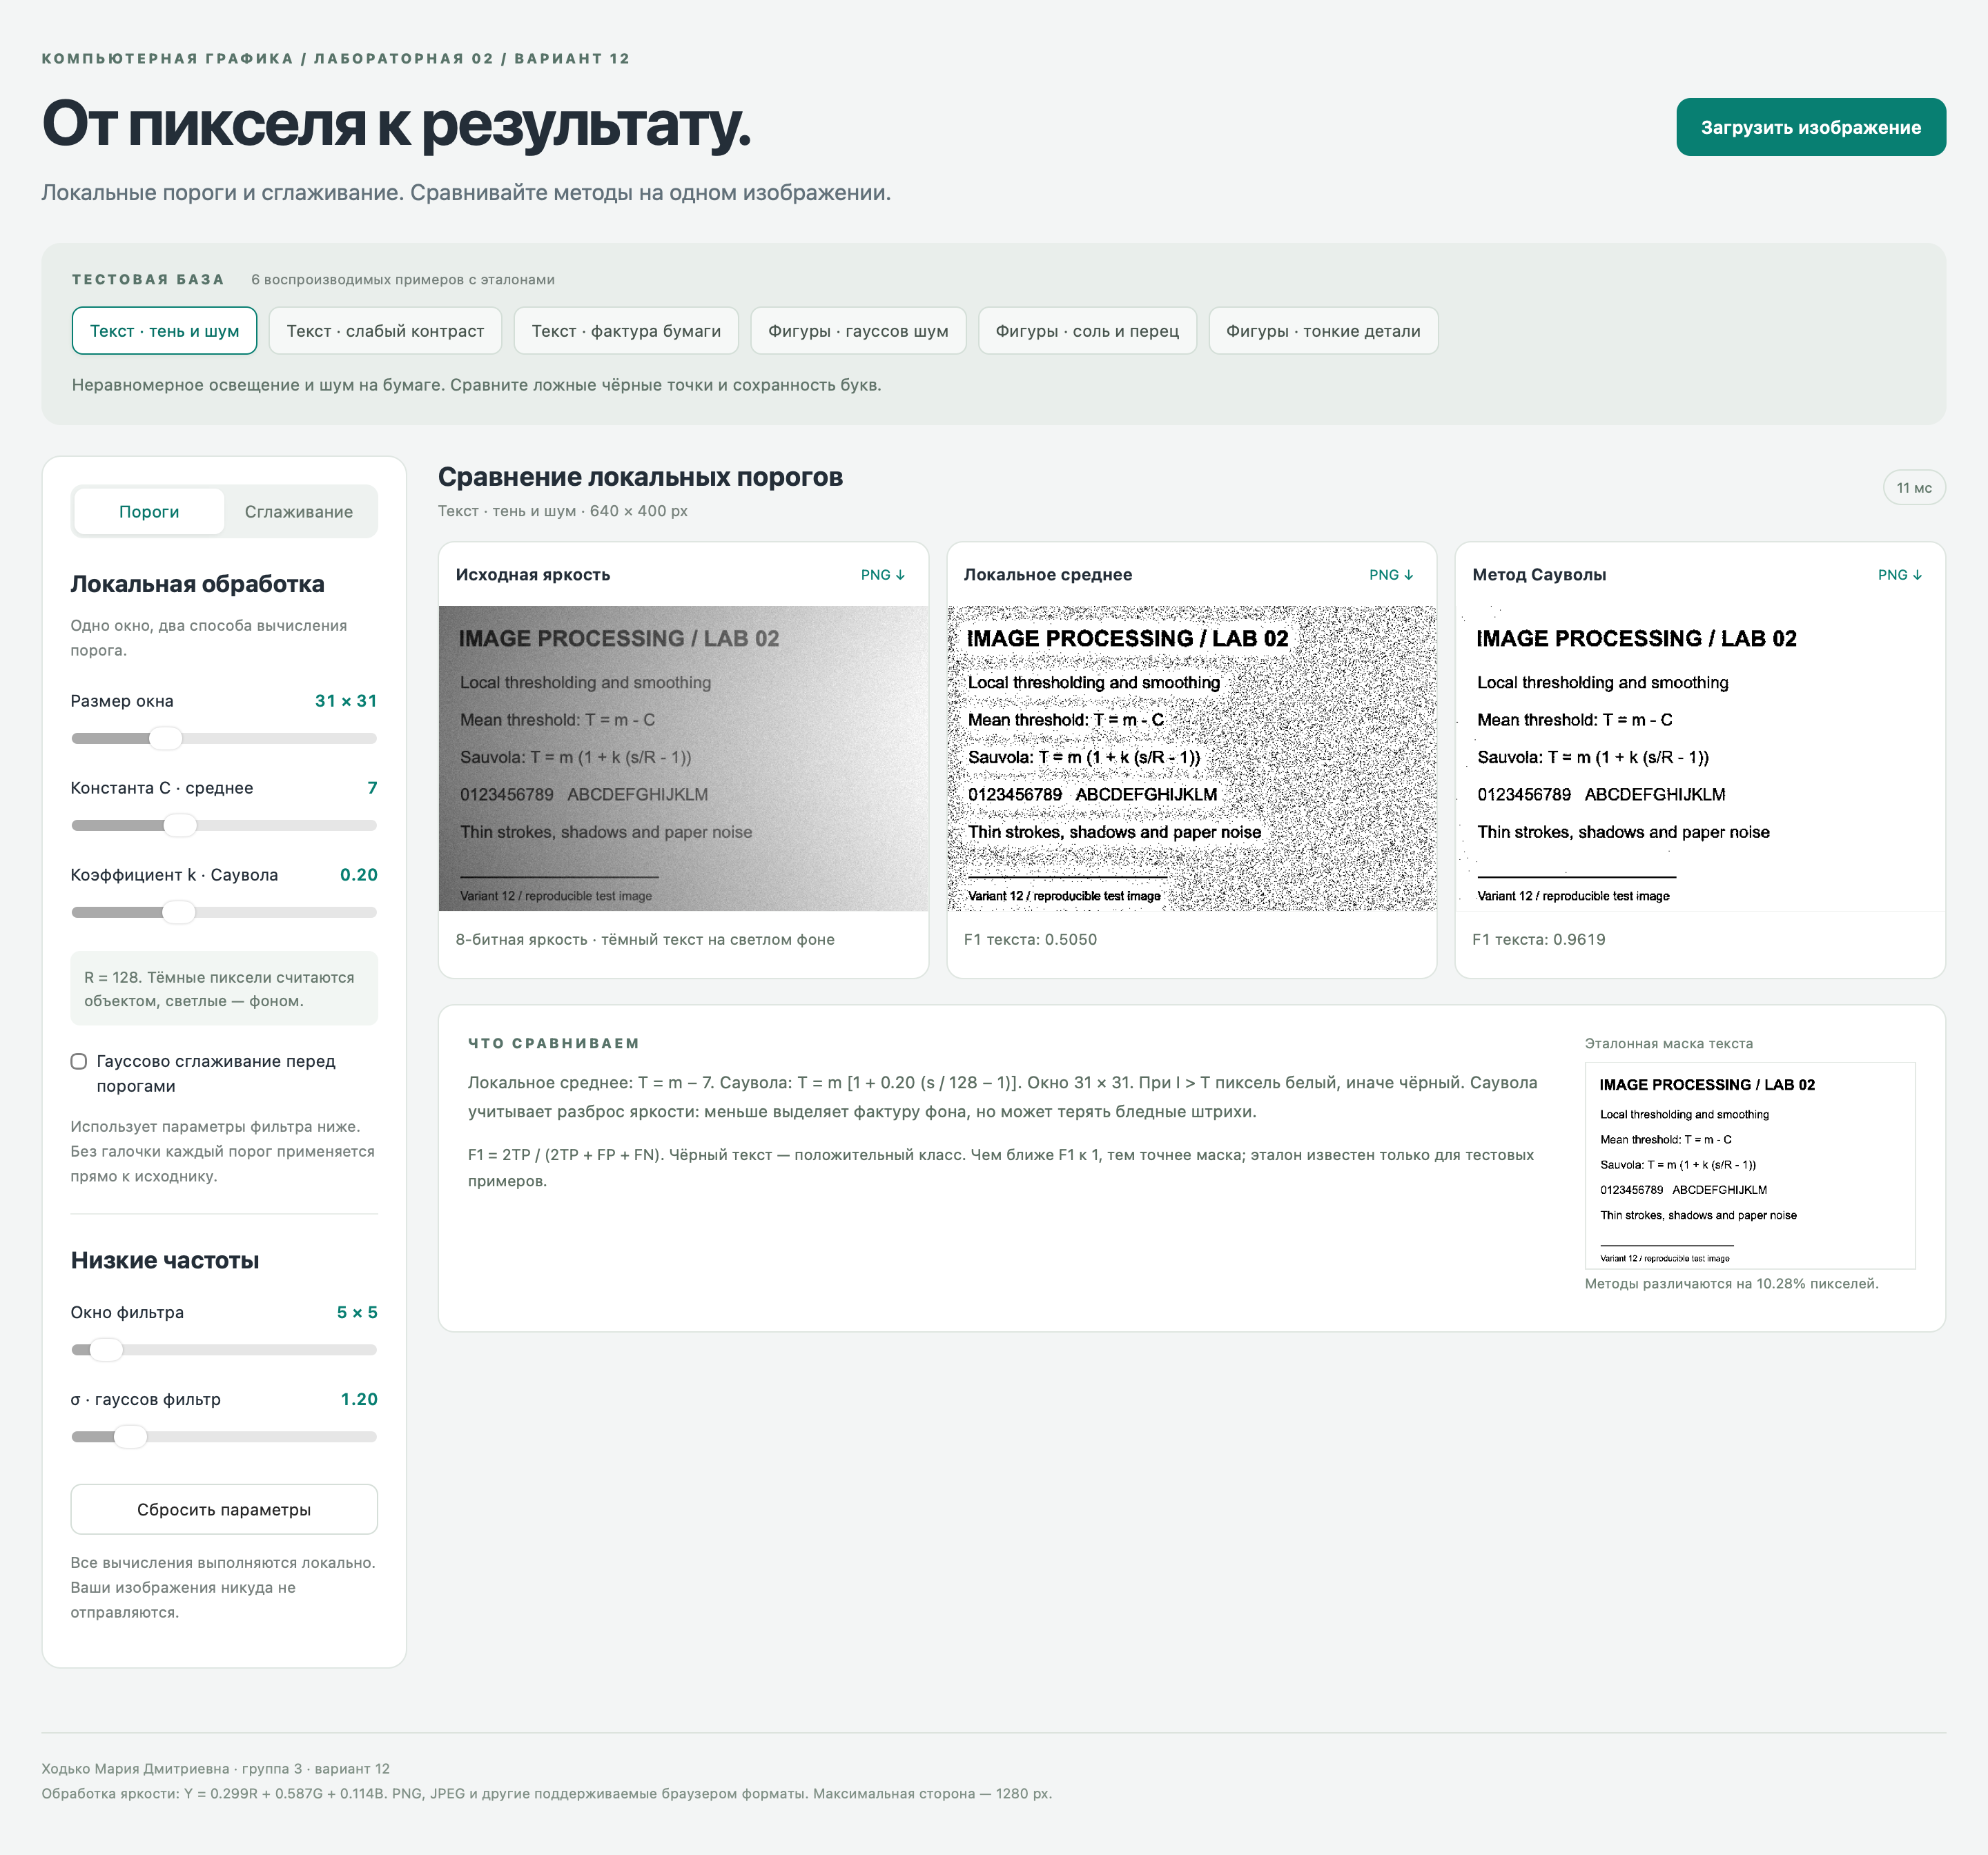
\includegraphics[width=\linewidth,height=0.43\textheight,keepaspectratio]{screenshots/01-threshold-shadow.png}
\caption{Режим локальной пороговой обработки: исходник, два результата, параметры и эталон.}
\vspace{6pt}
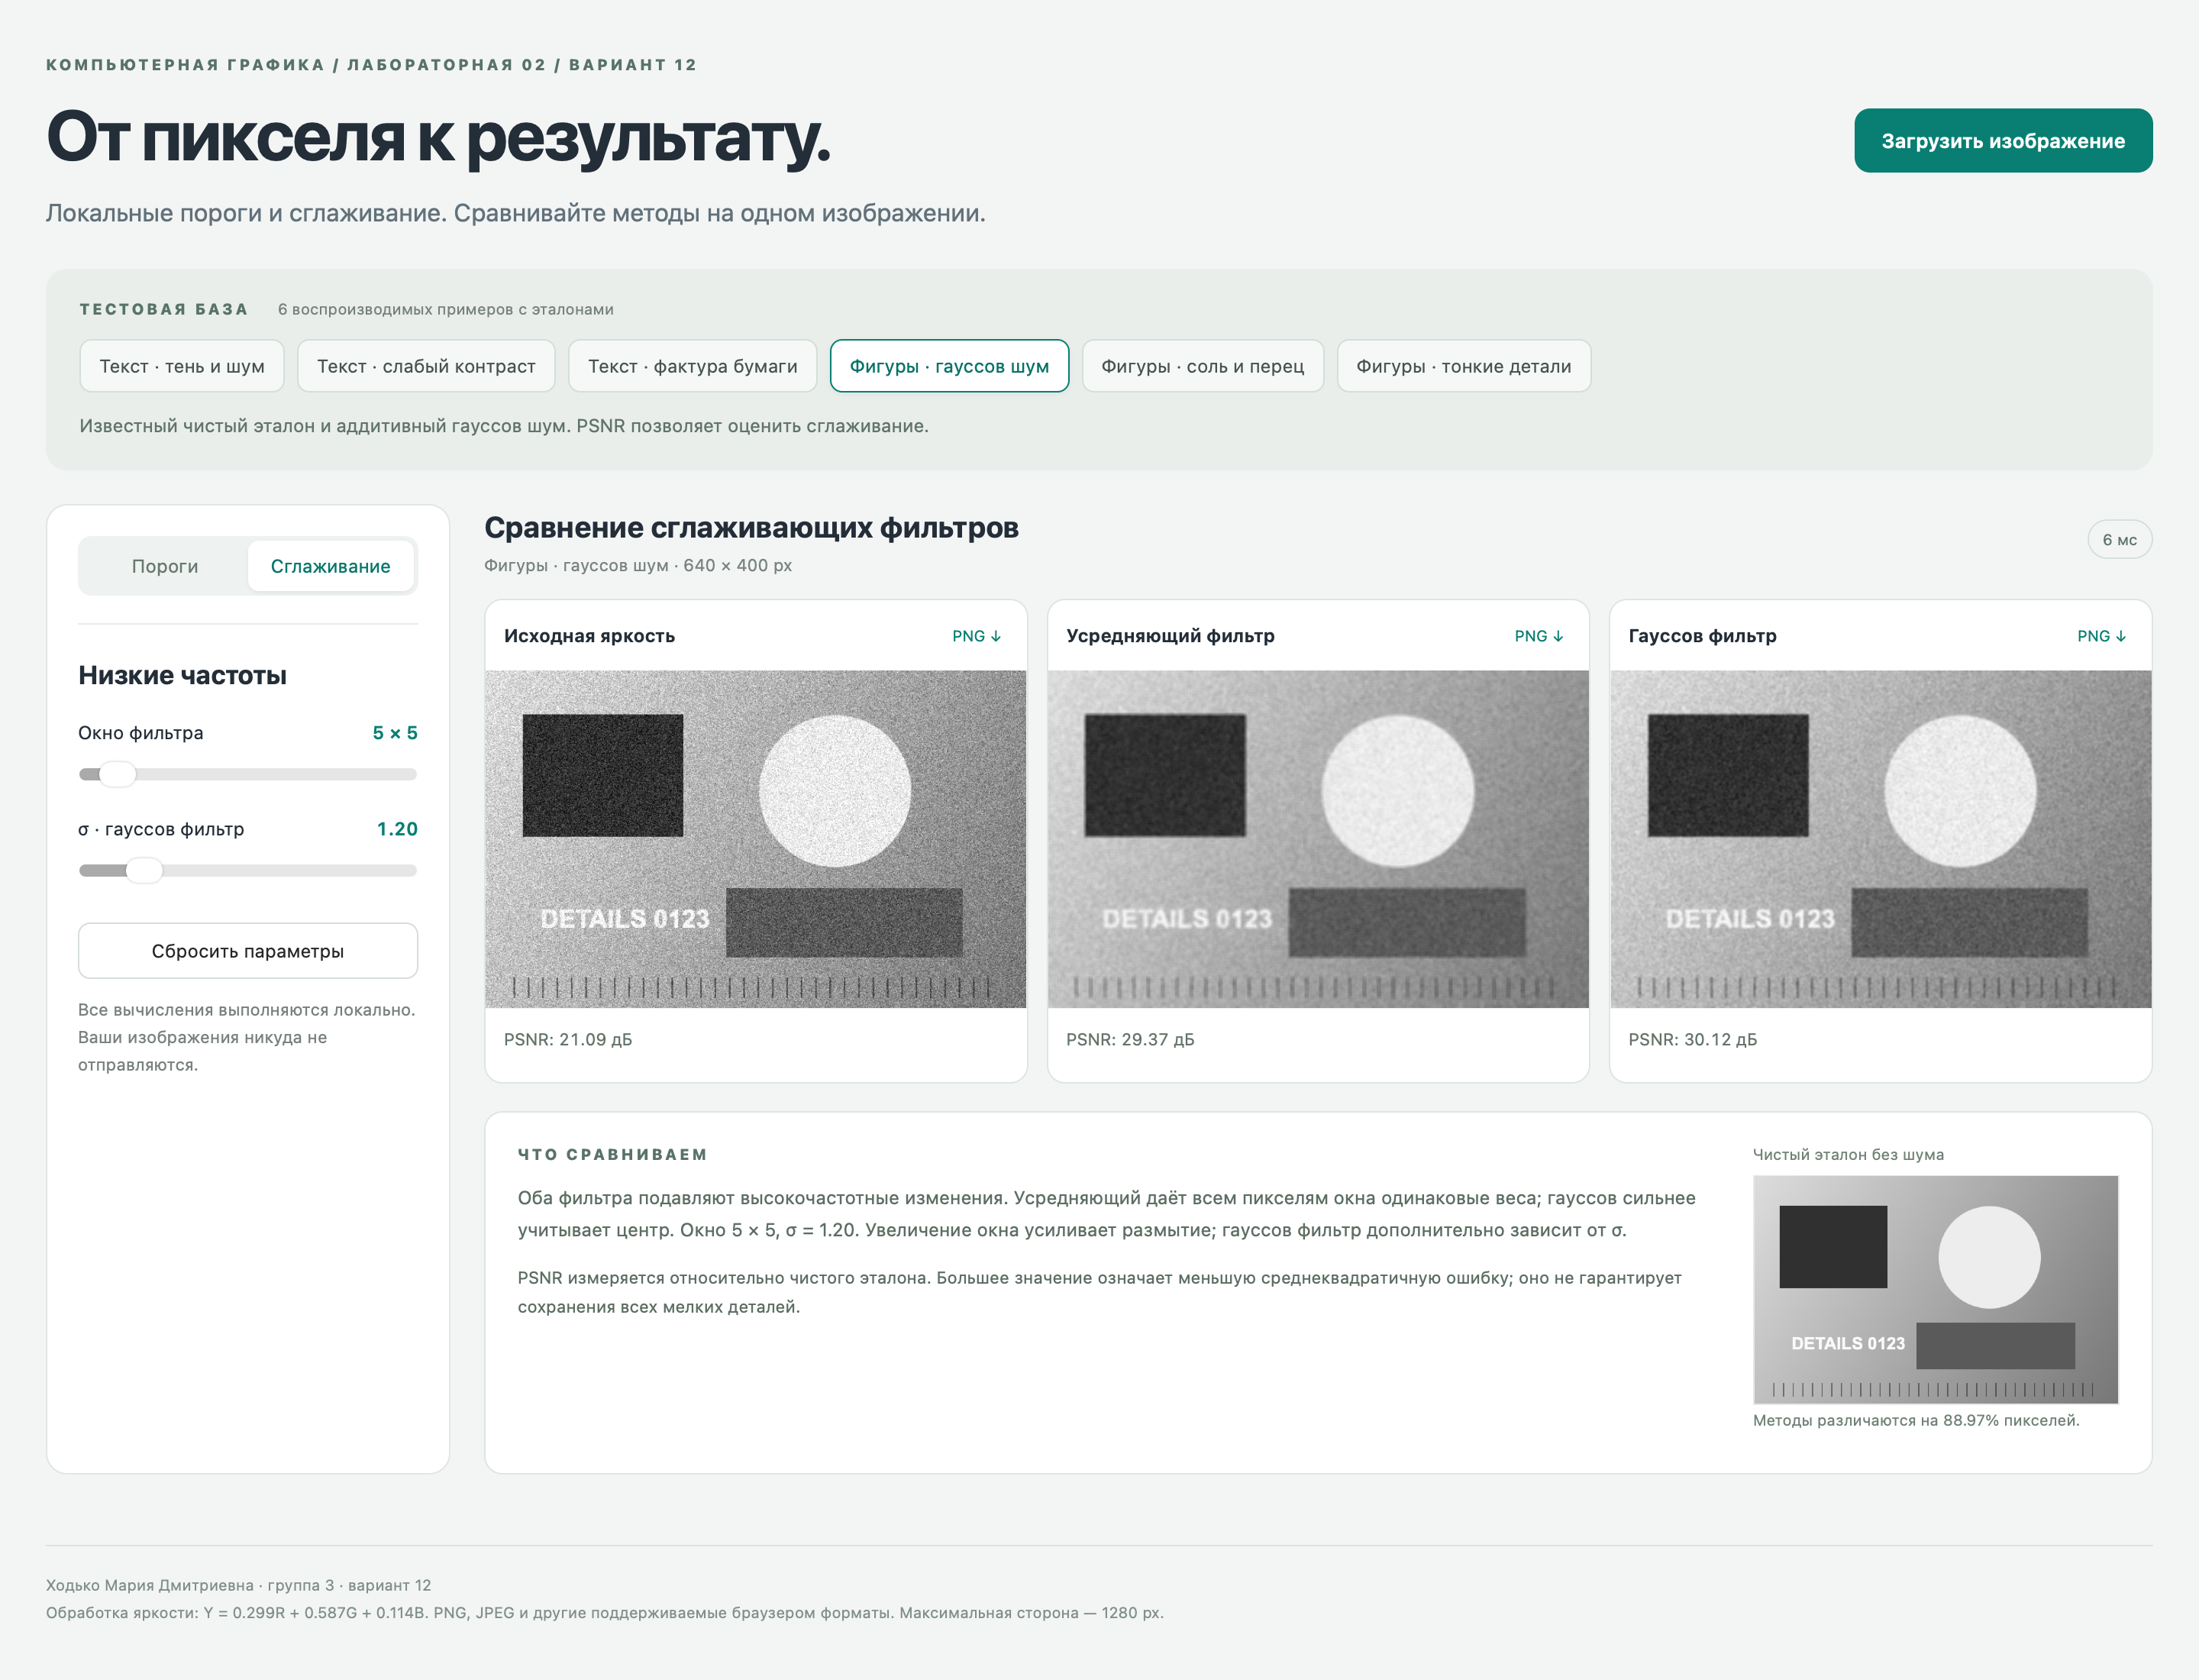
\includegraphics[width=\linewidth,height=0.34\textheight,keepaspectratio]{screenshots/04-smoothing-gaussian.png}
\caption{Режим сглаживания с оценкой PSNR относительно чистого эталона.}
\end{figure}

\section{Проверка корректности}
Автоматические проверки выполняют код приложения в JavaScriptCore. Пройдены восемь групп проверок: перевод в яркость и прозрачность; интегральные статистики против прямого подсчёта, включая края; сохранение константного изображения; численный пример усредняющего фильтра; симметрия, нормировка и центральный вес гауссова ядра; пороговые формулы и равенство порогу; F1, MSE и PSNR; отклонение некорректных параметров.

Дополнительно в WebKit пройдены девять проверок интерфейса: изменение ползунков, включение предварительного сглаживания, сохранение исходника, переключение режима, сброс параметров, загрузка и уменьшение PNG, перевод красного цвета в яркость, отсутствие ложной оценки качества без эталона и обработка повреждённого файла. Результаты сохранены в \texttt{results/ui-checks.json}, численные эксперименты --- в \texttt{results/metrics.json}.

\section{Вывод}
При выбранных параметрах Саувола лучше отделяет текст от шумного и фактурного фона, а локальное среднее лучше сохраняет бледные буквы. Сглаживание уменьшает шум ценой потери деталей: чем оно сильнее, тем больше размытие. Поэтому метод и параметры нужно подбирать под изображение.

\section*{Источники}
\begin{enumerate}
\item OpenCV. Image Thresholding: \url{https://docs.opencv.org/4.10.0/d7/d4d/tutorial_py_thresholding.html}.
\item scikit-image. Sauvola threshold: \url{https://scikit-image.org/docs/0.26.x/api/skimage.filters.html#skimage.filters.threshold_sauvola}.
\end{enumerate}
\end{document}
